
\chapter{Just-In-Time Compilation}
\label{ch:jitflow}

Experience integrating \FlowCore\ with the WebKit browser and visiting pages in the Alexa Top 1,000~\cite{alexa} revealed important issues about JavaScript's omnipresence on the Web.
In particular, that effort discovered that today's highly-interactive web applications rely on a performant JavaScript interpreter backed up by a just-in-time compiler.

Several recent approaches~\cite{vogt.etal+07,just.etal+11,groef.etal+12,kerschbaumer.etal+13} have shown that information flow tracking mitigates the shortcomings of current web security practices and successfully counters XSS-based information theft attacks.
Even though these dynamic tracking enhancements provide the desired security, all of the previous approaches suffer from the drawback of incurring performance penalties of at least 80\%.
Furthermore, they all integrate the tracking logic in the JavaScript interpreter, which itself commonly performs around four times worse than code generated by a just-in-time (JIT) compiler (\autoref{sec:jitflow-evaluation-performance}).

Currently, browser vendors compete for adoption by advertising JavaScript performance.
As a result of the ``browser wars,'' faster JavaScript virtual machines (VMs) now enable web applications with large amounts of JavaScript code.
Consequently, the slowdown seen when integrating information flow into the JavaScript interpreter represents a major obstacle to adoption.

The project that started \FlowCore\ answers this challenge by implementing dynamic information flow tracking in a JIT compiler.
The updated engine, \JitFlow, allows detection of suspicious network traffic that sends data to a server other than that intended by the application programmer.
The detection occurs at runtime, catching the code ``in flagranti'' when performing malicious actions such as data theft.

The work behind \JitFlow\ contributes:

\begin{itemize}

\item The first (to the best of my knowledge) dynamic information flow tracking engine in a JIT compiler for a dynamically typed programming language.

\item Several optimizations (\autoref{sec:jitflow-implementation}) essential to preserving the performance gains when JIT compiling the information flow tracking logic.

\end{itemize}

\section{The Threat of executing third Party Code}
\label{sec:jitflow-thirdpartycode}

The Same Origin Policy, still widely in use as a first line of defense in web applications, permits scripts access to methods and properties when sharing the same origin and restricts access otherwise.
Unfortunately, rules of the Same Origin Policy often clash with modern web application architecture, because the SOP only applies to cross-frame communication.
Previous experience with CrowdFlow~\cite{kerschbaumer.etal+13} shows that, within the Alexa top 500, some pages contain information influenced by code originating from up to six different domains is sent across domain boundaries.
Verification and proof that the mashup performs only the expected task and does not steal data is not available.
Hijacking just one commonly included script compromises the privacy of many web users~\cite{nikiforakis.etal+12}.

%------------------------------------------------------------------------------------------------------
\subsection{The Nature of Code Injection Attacks}
\label{sec:jitflow-codeinjection}

Because servers deliver JavaScript as source text, most content and third-party library providers compact their code by automatically shortening variable names, removing all extra whitespace as well as line breaks so the code becomes as small as possible.
This practice shortens the transfer time for loading JavaScript, but has the side effect of obfuscating the source code.
Web authors are unlikely to audit compressed code for security holes despite the fact that including it in the same execution context as the web application grants it access to application internals.
Consequently, a channel through which attackers can inject code that steals sensitive user information remains open and prevalent.

In addition to the risk of including such malicious third party code, I'd like to remind the reader of two other forms of code injection attacks.
Based on the method of injection, I distinguish between:

\begin{itemize}

\item \textit{Non-Persistent (Reflected) attacks}, that occur when the server sends client-provided code embedded in HTTP query parameters and HTML form submissions back to the user as page content after processing by the web application servers.

\item \textit{Persistent attacks}, that occur when the web application stores client-provided data server-side and reflects it back to subsequent visitors.

\end{itemize}
In both of these cases, from the client's perspective, the origin of the attacker code is the same as that of the web application itself, meaning that the Same Origin Policy can not prevent the attack.
Additional security requires a more powerful, behavior-focused mechanism, such as information flow tracking.

%------------------------------------------------------------------------------------------------------
\subsection{Threat Model}
\label{sec:jitflow-threatmodel}

As assumed when evaluating \FlowCore\ (\autoref{sec:first-class-evaluation}), I grant the attacker with the ability to inject code into a web application.
The attacker accomplishes injection by exploiting a XSS vulnerability or the ability to provide content for mashups, advertisements, libraries, etc. which other sites include.
To collect the stolen data, the attacker controls their own web host.
The attacker practices only code injection techniques and does not resort to packet sniffing, network interception, or control of the application servers.

%------------------------------------------------------------------------------------------------------
\subsection{Provided Security}
\label{sec:jitflow-providedsecurity}

The web browser running \JitFlow\ advanced significantly beyond the capabilities offered when evaluated with only the interpreter \FlowCore.
The updated browser protects against several information theft attacks, including, but not limited to:

\begin{itemize}[itemsep=4pt,parsep=4pt]

\item \textit{Sensitive Data Theft Attacks:}
By sending a GET request to a server under the attacker's control, the attacker can steal information in the URL of an image request:

\begin{snippet}
elem.src = "evil.com/pic.png?" + credit_card_number;
\end{snippet}

The attacker uses the request for the image as a channel to steal the user's credit card number as a payload in the GET request.
Merely changing the URL targeted by the \code{src} attribute of an image triggers loading of the image.

\item \textit{Keylogging Attacks:}
Similarly, to steal a username and password combination, an attacker might craft code that logs keystrokes by registering an event handler:

\begin{snippet}
document.onkeypress = listenerFunction;
\end{snippet}

The listener function records the user's keystrokes and sends them to the attacker's server through an HTTP request.

\item \textit{Cookie Stealing Attacks:}
Furthermore, if a script can access cookies, then an attacker can also steal a session cookie between the browser and an honest site by concatenating the \code{document.cookie} to the URL of the image request.
The stolen cookie allows the attacker to impersonate the user and hijack the user's session.

\end{itemize}

%------------------------------------------------------------------------------------------------------
\subsection{Sample Attack: Stealing Form Data}
\label{sec:jitflow-stealingformdata}

An HTML form provides a page with data entry fields that allow a user to enter text such as a username and password.
Once a user submits the form, the browser sends the data to the server.
Virtually all web applications rely on login fields to authenticate their users.
If an attacker manages to inject code into a web application that contains a login form, the attacker's script can read a user's credentials and send them to an attacker-controlled server.
Later, the attacker may use the stolen credentials to impersonate users of the web service.

\lstset{
  label=list:fieldinfo,
  caption={Example attack code that steals login form data from a web page.}
}
\begin{jscode}
// place hidden image on the page
var pixel = "<img src=\"http://www.attacker.com/pixel.png\"" +
            "id=\"pixel\" />";
document.write(pixel);

function stealFormData(type, value) {
  var payload = "url=" + document.domain + "&" + type + "=" + value;
  document.getElementById("pixel").src =
      "http://www.attacker.com/pixel.png?" + payload;
}

// add stealFormData to all forms on page
for (var i = 0; i < document.forms.length; i++) {
  for (var j = 0; j < document.forms[i].elements.length; j++) {
    var elem = document.forms[i].elements[j];
    elem.addEventListener("blur", // triggered when element loses focus
           function() { stealFormData(this.type, this.value) }, false);
  }
}
\end{jscode}

\autoref{list:fieldinfo} shows exploit code an attacker might use to steal credentials from the login form of a web page.
The attack script first loads an image (\codeline{2}) supplied by a server under the attacker's control.
The attacker designs the image to avoid perceptible changes in page layout.
Few users will notice the placement of a single transparent pixel, but the attacker can use the GET request as a channel to steal confidential page data whenever the image is reloaded from the server.

The attacker knows users will fill out the form and registers (\codelines{14}{15}) a \code{blur}-event handler on all forms elements on the page.
When a form element loses focus it triggers a call to the \code{blur}-event handler.
The handler, \code{stealFormData} defined on \codeline{5}, first encodes information about the page domain and contents of the form element which triggered the event in the \code{payload} variable.
Then it updates the \code{src} attribute of the image with a URL containing the payload.
This update causes the browser to automatically reload the image, sending the sensitive information in the URL of the image request.

\lstset{
  label={list:serverlogs},
  caption={Log of \code{attacker.com} from the running example.}
}
\begin{jscode}
[01/Jan/2014:21:34:10] "GET /pixel.png?url=www.bank.com&text=alice HTTP/1.1"
[01/Jan/2014:21:34:12] "GET /pixel.png?url=www.bank.com&password=bob69 HTTP/1.1"
\end{jscode}

By inspecting the server request logs, the attacker can reassemble the captured form data.
\autoref{list:serverlogs} contains some example entries of image requests.
The attacker can clearly identify a user of \code{www.bank.com} with login `\code{alice}' having the password `\code{bob69}'.

The webpage \textit{About The Open Web Application Security Project}~\cite{xsscheatsheet} hosts an extensive list of XSS vulnerabilities that provides a detailed description of all the different kinds of XSS attacks.

%xxxxxxxxxxxxxxxxxxxxxxxxxxxxxxxxxxxxxxxxxxxxxxxxxxxxxxxxxxxxxxxxxxxx

\section{Changes Made to the Information Flow Framework}
\label{sec:jitflow-framework}

Whether an interpreter or JIT-compiled code performs information flow tracking, the implementation requires supporting data structures and other modifications to the runtime VM.
\JitFlow\ makes some alterations to the underlying data structures that once supported \FlowCore.
Each modification focuses on increasing the performance of the tracking engine to support runtime compilation of code in \JitFlow.

\subsection{The Label Lattice}

Because \JitFlow\ forms the core of an information flow tracking web browser, it focuses on the ability to web map domains to security principals.
Previous experience~\cite{kerschbaumer.etal+12, kerschbaumer.etal+13} demonstrate that most web pages do not include more than 16 separate web origins.

\JitFlow\ retains the \FlowLabelRegistry, but reduces the number of bits used to represent a label.
The \FlowLabelRegistry\ still follows Myers' decentralized label model~\cite{myers.liskov+00} and represents security labels as a lattice join over domains (\autoref{fig:jitflow-label-lattice}).

\begin{figure}[ht]
 \centering
 \resizebox{\textwidth}{!}{
\begin{tikzpicture}[node distance = 1cm, auto,
    force/.style={rectangle, inner sep=5pt, text badly centered, minimum height=.8cm},
    every text node part/.style={align=center},
    ]

    \begin{scope}[yshift=4cm, xshift=-8cm]
    \node[shape=rectangle, draw] {
       \begin{tabular}{l|c}
          \multicolumn{2}{c}{\code{LabelRegistry} mapping} \\
          \hline
          \url{good.com} & \code{001} \\
          \url{other.com} & \code{010} \\
          \url{evil.com} & \code{100} \\
       \end{tabular}
    };
    \end{scope}

    \begin{scope}
    \matrix[nodes={force}, column sep=1cm, ampersand replacement=\&] {
        \node (ex) {\url{good.com} \\ \code{001}}; \&
        \node (mp) {\url{other.com} \\ \code{010}}; \&
        \node (ad) {\url{evil.com} \\ \code{100}}; \\
    };
    \end{scope}

    \begin{scope}[yshift=2cm]
    \matrix[nodes={force}, column sep=.5cm, ampersand replacement=\&] {
      \node (exUmp) {\url{good.com} $\sqcup$ \url{other.com} \\ \code{011}}; \&
      \node (exUad) {\url{good.com} $\sqcup$ \url{evil.com} \\ \code{101}}; \&
      \node (mpUad) {\url{other.com} $\sqcup$ \url{evil.com} \\ \code{110}}; \\
    };
    \end{scope}

    \begin{scope}[yshift=4cm]
    \matrix[nodes={force}, column sep=1cm] {
      \node (exUmpUad) {\url{good.com} $\sqcup$ \url{other.com} $\sqcup$ \url{evil.com} \\ \code{111}}; \\
    };
    \end{scope}

    \begin{scope}[yshift=-2cm]
    \matrix[nodes={force}, column sep=1cm] {
      \node (bot) {interpreter \\ {$\bot$}}; \\
    };
    \end{scope}

    \draw[arrow] (ex) -- (exUmp);
    \draw[arrow] (ex) -- (exUad);

    \draw[arrow] (mp) -- (exUmp);
    \draw[arrow] (mp) -- (mpUad);

    \draw[arrow] (ad) -- (exUad);
    \draw[arrow] (ad) -- (mpUad);

    \draw[arrow] (exUmp) -- (exUmpUad);
    \draw[arrow] (exUad) -- (exUmpUad);
    \draw[arrow] (mpUad) -- (exUmpUad);

    \draw[arrow] (bot) -- (ex);
    \draw[arrow] (bot) -- (mp);
    \draw[arrow] (bot) -- (ad);

\end{tikzpicture}
}
  \caption{Example Label Lattice for domains \url{good.com}, \url{other.com}, and \url{evil.com}}
  \label{fig:jitflow-label-lattice}
\end{figure}

It stores a mapping from web security principals (domain name strings) to unique bit positions.
Taken as a whole, these bit positions form a bit vector that acts as a confidentiality label, holding up to 16~different domains.

\subsection{Encoding Labels}
\label{sec:jitflow-labelencoding}


The \FlowCore\ interpreter, already achieves high performance by using a type-tagged union, called \jsvalue, to represent immediate values, object references, and numbers.
However, the fat value extension from 64-bit \jsvalues to 128-bit entities that join a value and label tag, proved itself too radical a change for the JavaScriptCore's JIT engine.
Fat values required updating offset calculations scattered throughout the code base.

\begin{figure}[ht]
  \centering
\begin{tabular}{cccc|l}
    \multicolumn{4}{c|}{bit values} & type  \\
\hline
    \code{0000} & \code{xxxx} & \code{pppp} & \code{ppp0} & \code{pointer} \\
\hline
    \code{0000} & \code{xxxx} & \code{0000} & \code{0000} & \code{empty} \\
    \code{0000} & \code{xxxx} & \code{0000} & \code{0002} & \code{null} \\
    \code{0000} & \code{xxxx} & \code{0000} & \code{0004} & \code{deleted} \\
    \code{0000} & \code{xxxx} & \code{0000} & \code{0006} & \code{false} \\
    \code{0000} & \code{xxxx} & \code{0000} & \code{0007} & \code{true} \\
    \code{0000} & \code{xxxx} & \code{0000} & \code{000a} & \code{undefined} \\
\hline
    \code{FFFF} & \code{xxxx} & \code{iiii} & \code{iiii} & \code{integer} \\
\hline
    \code{0001} & \code{dddd} & \code{dddd} & \code{dddd} & \tikzmark{2nd} \multirow{3}{*}{\code{  double}} \\
    \code{\vdots} & & & & \\
    \code{FFFE} & \code{dddd} & \code{dddd} & \code{dddd} & \tikzmark{4th} \\
\hline
     \tikzmark{p1}\code{~~~}\tikzmark{p2} & \tikzmark{p3}\code{~~~}\tikzmark{p4} & \tikzmark{p5}\code{~~~}\tikzmark{p6} & \multicolumn{1}{c}{\tikzmark{p7}\code{~~~}\tikzmark{p8}} & \multicolumn{1}{l}{\tikzmark{p9}} \\
     & & \tikzmark{v1}\code{~~~~} & \multicolumn{1}{c}{\code{~~~~}\tikzmark{v2}} & \multicolumn{1}{l}{} \\
     & \tikzmark{l1}\code{~~~~}\tikzmark{l2} & \multicolumn{2}{c}{} \\
     \tikzmark{t1}\code{~~~~}\tikzmark{t2} & \multicolumn{3}{c}{} \\
\end{tabular}
\begin{tikzpicture}[overlay, remember picture]
    \draw [decoration={brace,amplitude=.5em}, decorate]
    ($(2nd)+(0,1ex)$) -- ($(4th)+(0,1ex)$);

    \draw [|-|] ($(v1)$) -- ($(v2)$) node[anchor=west]{Value};
    \draw [|-|] ($(l1)$) -- ($(l2)$) node[anchor=west]{Label Encoding};
    \draw [|-|] ($(t1)$) -- ($(t2)$) node[anchor=west]{Type Information Tag};
    \node [font=\tiny] at ($(p1)$) {63};
    \node [font=\tiny] at ($(p2)$) {48};
    \node [font=\tiny] at ($(p3)$) {47};
    \node [font=\tiny] at ($(p4)$) {32};
    \node [font=\tiny] at ($(p5)$) {31};
    \node [font=\tiny] at ($(p6)$) {16};
    \node [font=\tiny] at ($(p7)$) {15};
    \node [font=\tiny] at ($(p8)$) {0};
    \node [anchor=west, font=\tiny] at ($(p9)$) {bit position};
\end{tikzpicture}
\caption{
   \label{fig:jitflow-bit-encoding}
   Label encoding using bits 32--47 of \jsvalues, supporting 16 security principals.
}
\end{figure}

\JitFlow\ implements an \term{inline label} approach not previously considered (\autoref{sec:implementation}).
Rather than extending the size of the \JSValue\ data type, it repurposes 16 of the bits to hold the security label.
This modification allows for a low performance overhead encoding that packs both the label and the typed value within the same 64~bit word, avoiding a change to any offset and layout calculations in the JIT compiler.

Because the repurposing of bits affects the interpretation of the \JSValue, it pays to examine each case:

\begin{description}

\item[Pointers/Immediates:]
\jsvalues\ starting with the highest 16~bits all set to~zero (\autoref{fig:jitflow-bit-encoding}) indicate either a pointer or immediate type.
The VM uses the lowest four bits to distinguish pointers from immediates.
Pointers have alignment with these bits all set to~zero, while immediate values hold non-zero entries in the same lowest four bits: \code{empty:0x00}, \code{null:0x02}, \code{deleted:0x04}, \code{false:0x06}, \code{true:0x07}, and \code{undefined:0x0a}.

\item[Pointers:]
In JavaScriptCore, pointer addresses occupy 46~bits (bits 0--47).
Unfortunately, this design does not leave any space to directly encode a label within \jsvalues.
Hence, \JitFlow\ modifies allocation of the garbage-collected heap so that it fits within a 32~bit address space.
This change limits the heap to be 4GB in size, but frees 16 bits of JavaScript object references for a security label (bits~32--47, marked as \code{xxxx} in \autoref{fig:jitflow-bit-encoding}).
This modification allows encoding of up to 16 different domains and permits efficient bit arithmetic for the frequent label join operation, an essential implementation detail for performance when propagating information flow.
At the expense of maximum heap size, \JitFlow\ gains an efficient labeling of virtual machine values.

\item[Integers:]
Values starting with the highest 16~bits all set to~one indicate an integer value type.
ECMAScript~\cite{ecma} specifies that the JavaScript operators only deal with 31~bit integers, leaving bits 32--47 unused by the original WebKit encoding.
This arrangement means that same set of bits as used previously in pointers and immediates remain free for encoding a label on integers.

\item[Doubles:]
Doubles in the ECMAScript specification follow the double-precision 64~bit format as specified in the IEEE Standard for Binary Floating-Point arithmetic~\cite{ieee754}.
Therefore, WebKit reserves all values with highest 16~bits between \code{0x0001} and \code{0xfffe} for doubles.
Unfortunately, this encoding uses all available bits for the double value, leaving no room for a label.
To compensate for this shortcoming, \JitFlow\ treats doubles conservatively by implicitly tagging them with the highest security label in the lattice.
This decision makes double values a source of label creep.

\end{description}

\subsection{Tracking Data Flow}
\label{sec:jitflow-tracking-dataflow}

Code and data originally tagged with different security principals (web domains) may interact during execution of a JavaScript program.
The encoding of labels within the lattice supports tagging a single value as having been influenced by multiple principals.
For every operation, \JitFlow\ inspects the labels of all inputs, including the current program counter.
As described in \autoref{ch:label-tracking}, it constructs a label representing the lattice join over all arguments and the current execution context.
\JitFlow\ then attaches the resulting label to the operation's output value.

For an example of a situation where two principals influence a single value (simplified to omit the current execution context), consider the code snippet:

\begin{snippet}
pub += secret;
\end{snippet}

where the variable \code{secret} originates from domain \code{good.com} (\code{001}) and the variable \code{pub} originates from domain \code{evil.com} (\code{100}).
To construct a label that represents this confluence, the \JitFlow\ performs a label join operation (via bitwise or) to obtain the join of the domains \code{good.com}~$\sqcup$~\code{evil.com} (\code{001|100}).
The updated variable \code{pub} then carries the resulting label (\code{101}).


\subsection{Tracking Control Flow}
\label{sec:jitflow-tracking-controlflow}

\JitFlow\ inherits the same technical difficulties regarding the semantics of the JavaScript language that \FlowCore\ addressed.
The lack of static typing pushes \JitFlow\ to use the same control flow stack for propagating the influence that a branch in control flow has over operation within the branch.
\JitFlow\ uses \FlowCore's parser to emit the \dup, \join, and \popj instructions that assist in tracking control-flow joins and branches as the program executes.
It allocates space for the program counter stack of a function during setup of each JavaScript stack frame.

In JavaScript, loop induction variables declared with the \code{var} keyword reside in the function scope and remain accessible outside of the loop which they control.
As shown in \autoref{list:jitflow-stealpin-source}, an attacker can use this feature to construct a correspondence between the induction variable (labeled lower in the security lattice) and a confidential value (labeled higher in the lattice) by breaking out of the loop.
Once the loop has terminated early, the attacker returns the induction variable (still labeled lower in the lattice) and leaks the value of the confidential variable.

\lstset{
  caption={Inferring the value of the variable \code{secret} by observing the change in control flow using an active implicit information flow.},
  label={list:jitflow-stealpin-source}
}
\begin{jscode}
function stealpin(secret) {
  for (var i=0; i < 10000; i++) {
    if (i == secret)
      break;
  }
  return i;
}
\end{jscode}

As explained in Chapters \ref{ch:instructions} and \ref{ch:label-tracking}, JavaScript complicates the context tracking issue by supporting labeled \code{break} and \code{continue} statements that cause early exit from arbitrarily nested inner loops.
When a program performs one of these scope-jumping actions, all further operations carried out within the function become tagged with the label under which the break or continue occurred.
\JitFlow\ accomplishes this tracking using the same mechanism as \FlowCore: a stack of labels that follow the program counter label, and issuance of a \popj instruction to upgrade the function's entire control flow stack.
\autoref{list:jitflow-stealpin-bytecodes} contains the instruction sequence for the \code{stealpin} function shown in \autoref{list:jitflow-stealpin-source}.

\lstset{
}
\begin{figure}[h]
\begin{python}
code = r'''
function stealpin(secret) {
  for (var i=0; i < 10000; i++) {
    if (i == secret)
      break;
  }
  return i;
}

print(debug(stealpin))
'''
import sys
sys.path.append('..')

import jsc
j = jsc.jsc(code)
j.run()

import bytecodeformatter
bytecodeformatter.tikz_picture(j.instructions())
\end{python}
  \caption{Instruction sequence of the \code{stealpin} function in \autoref{list:jitflow-stealpin-source}.},
  \label{list:jitflow-stealpin-bytecodes}
\end{figure}

Immediately after entry, the \code{stealpin} function contains a loop that begins with the \dup\ instruction (\bcodeline{01}) that pushes a new security scope for the loop body.
JavaScriptCore places the condition at the end of the loop body, so the \join\ instruction that upgrades the security scope corresponding to the loop belongs on \bcodeline{31}.
After evaluating the condition, the loop body begins at \bcodeline{07}.

The loop body consists of an \code{if}-statement that acts as a nested security scope.
This scope begins with a \dup\ instruction (\bcodeline{07}) and gets upgraded (\bcodeline{12}) after evaluation of the conditional (\bcodeline{08}).
Should the condition fail, control flow branches to \bcodeline{22} which pops a label off the control flow stack indicating the end of the \code{if}-statement.
When the condition succeeds, the body of the \code{if} executes the \code{break} statement.
A \popj\ instruction (\bcodeline{17}) precedes the jump (\bcodeline{20}) that directs control flow out of the loop.
This instruction causes \JitFlow\ to pop the scope corresponding to the \code{if}-statement (argument \code{pop:1}) and to upgrade two levels below it (argument \code{join:2}), corresponding to the loop body and the function itself.

Regardless of the path through the loop, finishing with the normal exit or by following the \code{break} statement, the loop ends with a \popj\ instruction (\bcodeline{36}) that restores the control flow stack to the level it had before loop entry.

\subsection{Browser Integration}

Solely tracking the flow of information within the JavaScript engine only provides limited security against data theft attacks.
The DOM, for example, provides an interface that allows JavaScript in a web page to reference and modify HTML elements as if they were JavaScript objects.
Attacker-supplied JavaScript code can use the DOM as a communication channel for stealing information present in a web page.
\JitFlow\ prevents such data theft attempts by labeling DOM objects based on the origin of their elements and attributes.
This work focuses solely focus on JIT-compiling the information flow tracking logic within the JS-engine and the accompanying performance gain.
Kerschbaumer~et.~al.~\cite{kerschbaumer.etal+13} describes interaction of browser subsystems with the JS-engine.

\section{JIT Implementation of Information Flow}
\label{sec:jitflow-implementation}

This section presents the lower-level implementation which allows the JIT compiler to perform this tracking at substantially improved speeds.
The \JitFlow\ implementation, including \FlowLabelRegistry\ and other data structures shared with \FlowCore, adds approximately 4,000 lines of C++/assembly code to WebKit's codebase.\footnote{
Calculated by performing a \texttt{git diff base | grep "\textasciicircum+[\textasciicircum+]" | wc -l}}

\subsection{Encoding Labels}
\label{sec:jitlabelencoding}

When implementing information flow logic in the JIT compiler, native functions impose an additional design constraint.
JavaScriptCore's JIT compiler interpreter require a unified representation that supports passing \jsvalues\ between native functions (implemented in C++) and JIT-compiled JavaScript functions.
The \term{inline label} representation results in high performance, so \JitFlow\ modifies the \JSValue\ representation as detailed in \autoref{sec:jitflow-labelencoding}.
The label resides in bits 32--47 of integers, pointers, and immediates, while doubles remain implicitly labeled with the highest available label in the lattice.

\subsection{Tracking Data Flow in the JIT}
\label{sec:jitdataflow}

\FlowCore\ modifies JIT compiler in JavaScriptCore to track information flow in all binary operations:  \code{add}, \code{sub}, \code{mul}, \code{div}, \code{mod}, \code{lshift}, \code{rshift}, \code{urshift}, \code{bitand}, \code{bitor}, and \code{bitxor}.
Because JavaScript semantics allow for ad-hoc polymorphism, i.e., using the arithmetic add operator to perform both, numeric addition and string concatenation, the \code{add} operation supports multiple data types.

\lstset{
  caption={Label propagation for the numeric \code{add} instruction, with left and right integer operands in registers \code{RAX} and \code{RBX} respectively.
  Registers \code{R11} and \code{R12} serve as scratch registers for computing the labels encoded in bits 32--47.},
  label={list:jitflow-propagation},
}
\begin{asmcode}
// to join the labels of RAX and RBX
// move the first value (including label) into scratch register
MOV R11, RAX
// then bitwise-or first value (including label) with second value
OR  R11, RBX

// to join the cached top of the label stack
// first load the cached top-label of the pc-stack into scratch register
MOV R12, [RSP+60h]
// then bitwise-or the top-label of the pc-stack with operand labels
OR  R11, R12

// mask out value bits, so only label bits remain in R11
// first load the label-bit-mask into scratch register
MOV R12, 0FFFF00000000h
// then bitwise-and label-bit-mask with accumulated label
AND R11, R12

// perform the 32-bit add operation
ADD EBX, EAX
// bitwise-or the result with the joined label
OR  RBX, R11
\end{asmcode}

\autoref{list:jitflow-propagation} illustrates how the JIT compiler performs label propagation, by providing a simplified portion of the assembly code emitted by the JIT compiler for integer addition.
The binary operation has been split into three parts to give a precise description of each computation step:

\begin{enumerate}

\item \textit{Joining Operand Labels:}
As illustrated, \code{RAX} holds the left operand and \code{RBX} holds the right operand.
Registers \code{R11} and \code{R12} serve as scratch registers for the label propagation calculation.
Because the calculation of the addition and the propagation of the label must be kept separate, the code first copies the value of the left operand (including its label) into register \code{R11} (\codeline{2}).
Without masking out the label, \JitFlow\ joins in the value (and label of) the right operand using a bitwise-or (\codeline{3}).
At this point, \code{R11} contains the join of the labels of both operands together with the bitwise-or of the values.

The label on the result of the addition must also include the label from the current context.
Because the top of the control flow stack provides the security context to every binary operation, \JitFlow\ caches it in the \code{JITStackFrame} (\autoref{sec:jitcontrolflow}).
Line~6 retrieves the label from the cache into register \code{R12}.
The VM joins in this context label using another bitwise or, accumulating the result in register \code{R11} (\codeline{7}).

Register \code{R11} now contains the final label that will be attached to the result of the addition.
However, some non-label bits within the register are non-zero, as a result of using the operand values directly.
Unfortunately, x86\_64 architecture does not support 64~bit immediate operands for the bitwise and operator, so masking out the value bits requires two steps.
First, \JitFlow\ loads a label mask, which has only bits 32--47 set to one, into register \code{R12} (\codeline{10}).
Next, the mask and accumulated label undergo bitwise and, leaving only the label's bits active in register \code{R11} (\codeline{11}).

\item \textit{Performing the Operation:}
After calculating the label, the \JitFlow\ performs the addition of the two operands (\codeline{13}) with a 32~bit add instruction.
For simplification, the example elides an overflow check that occurs immediately after the addition.
In practice, this check makes use of the overflow and carry flags and transfers control to a slow path that coerces the input integers into doubles.

\item \textit{Assigning the Accumulated Label:}
Assuming the addition finished without overflow, the last step combines the accumulated label and the computed result value.
\JitFlow\ does not have to mask out any active bits within the label field of the result value before the label assignment because of two observations.
First, the addition operation is 32~bits and only affects the value portion, not the label field.
Second, any active label bits in the result come from an input operand and form a strict subset of the active bits in the accumulated label (register~\code{R11}).
Together, these properties allow \JitFlow\ to use bitwise-or to apply a label to the result value in register \code{RBX} (\codeline{15}).

\end{enumerate}

\subsection{Optimizing Control Flow Tracking in the JIT}
\label{sec:jitcontrolflow}

The steps taken to increase JIT compiler performance for tracking control flow involved successive refinement.
For example, JavaScriptCore's JIT compiler does not fully implement all of the bytecode instructions and often calls back into the interpreter to handle slow paths.
At one stage during development, the \JitFlow\ compiler implemented our the new control-flow instructions (\autoref{ch:instructions}) through a callback to C++.
This stage of implementation naturally had a higher performance overhead than the final product.

\JitFlow\ uses three techniques to enable fast tracking of control-flow influence:
\begin{enumerate}

\item \textit{It pre-allocates memory for the control-flow stack}, just as an unmodified JavaScriptCore pre-allocates an array for the call-frame stack.
Rather than allocating a small control-flow stack for each function frame, which negatively impacts runtime performance, each JavaScript function call now reserves space on a global control-flow stack for the number of labels that it requires for worst-case nesting depth.
Reservation of this space is as simple as incrementing a stack pointer in the pre-allocated array, analogous to bump allocation in memory management.

\item \textit{It caches the top label of the control-flow stack.}
Ordinarily, the information-flow tracking VM finds the label of the current execution context by following a chain of references that starts at the \code{CallFrame} pointer in the current \code{StackFrame}, traverses through the control-flow stack pointer in the current \code{CallFrame} and finally ends at an offset from the base of the current control-flow stack.
Because all data-flow operations also join in the current program counter label, \JitFlow\ caches the top of the control-flow stack in the \code{StackFrame} data structure so that it remains accessible through a fixed offset from the \code{StackFrame}.
\autoref{fig:jitflow-stackframe} shows both the chain of references and the cache location.

\begin{figure}[ht]
  \centerline{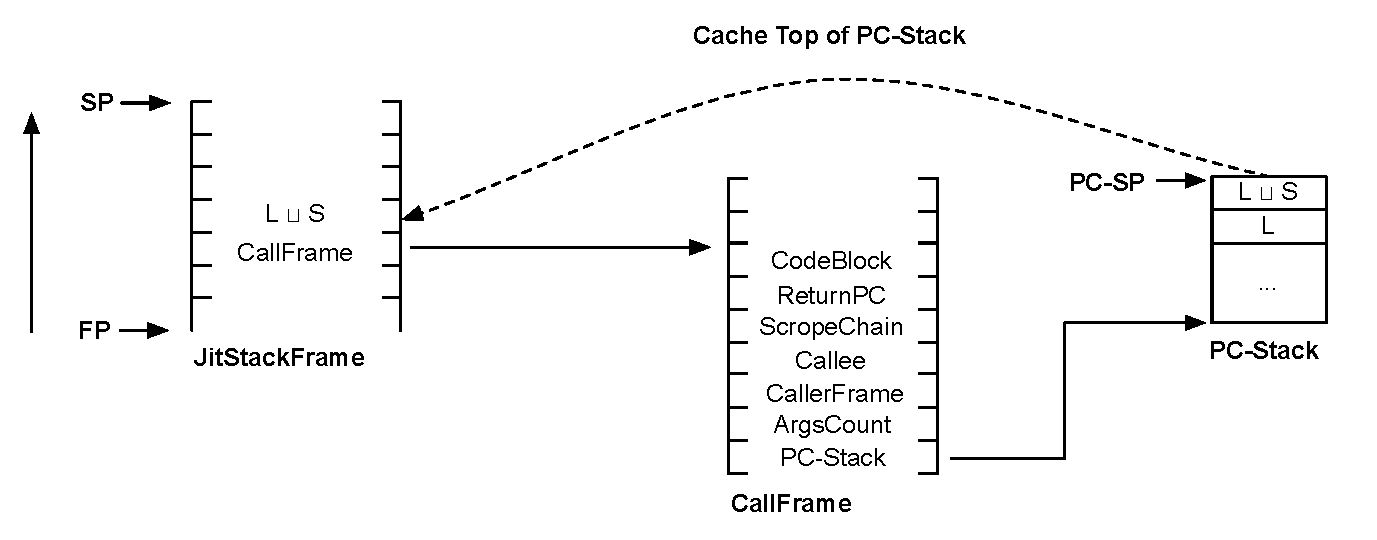
\includegraphics[width=\linewidth,keepaspectratio=true]{graphics/stackframe.pdf}}
  \caption{Interaction of native \code{JITStackFrame}, \code{CallFrame}, and Control-flow stack.}
  \label{fig:jitflow-stackframe}
\end{figure}

\JitFlow\ updates this cache every time the top label of the control-flow stack changes.
This update occurs at control-flow branches and joins and is less frequent than the data-flow operations that access the top label.

Additionally, using such a caching mechanism allows \JitFlow\ to avoid expensive updates on top of the control-flow stack if the label of the predicate and the cached label are identical.
As previously mentioned, the instruction \join\ upgrades the top of the control-flow stack by joining it with the label of the predicate value.
To avoid such unnecessary updates, \JitFlow\ emits compiled code that first checks the equality of the cached label in the \code{JITStackFrame} and the label of the predicate.
If so, the runtime system skips the expensive task of following the pointers to update the top of the control-flow stack because it already holds the correct label.

\item \textit{It implements the instructions that maintain the control-flow stack directly in assembly.}
\JitFlow\ takes as input the same instruction stream as the \FlowCore\ interpreter.
When the JIT compiler encounters one of the control-flow stack manipulation instructions (\autoref{ch:instructions}) it emits assembly code that performs the operation.
Not only does this code access the control-flow stack through the appropriate reference path shown in \autoref{fig:jitflow-stackframe}, but it also updates the cached top label when necessary.
Cache updates only occur in the \join\ and \popj\ instructions, because the \dup\ instruction modifies stack height but does not change the label on top.

Implementing the instructions that maintain the control-flow stack (\dup, \join, and \popj) in assembly code avoids expensive callbacks into C++ at runtime, allowing \JitFlow\ to increase speed by not having to (i) save and restore registers when calling into C++ and (ii) perform the expensive trampoline jump to find the function entry point in C++.

\end{enumerate}

Only by implementing all of these techniques was \JitFlow\ able to achieve the low-overhead performance measured in \autoref{sec:jitflow-evaluation}.

\section{Evaluation}
\label{sec:jitflow-evaluation}

This section evaluates the performance gained by implementing the logic for dynamically tracking information flow in JIT-compiled code.
The techniques used to validate that the implemented logic correctly tracks the flow of information also deserve emphasis.
Finally, I distinguish the limitations that arise as implementation artifacts from the fundamental limitations of the information flow approach.

WebKit contains an interpreter, JavaScriptCore (JSC), that executes a bytecode instruction sequence using direct threaded interpretation\footnote{
In March 2012, JavaScriptCore changed to a low-level interpreter, implemented via a custom language that generates the assembly for a direct threaded interpreter.
The benchmarks shown here measure the performance of the C++ version of JSC that predates this change.
}.
The WebKit project also contains a template JIT compiler that compiles the bytecode instruction stream and an optimizing JIT compiler based on a program's data-flow graph.
\JitFlow\ builds upon the template JIT and does not implement information flow in the optimizing JIT compiler, which operates only on Macintosh operating systems.
All of the following benchmarks compare information flow implementations of interpreter-only and JIT-only execution modes.

\begin{table}[ht]
\centering
\resizebox{\columnwidth}{!}{
\begin{tabular}{r l l l}
\textit{Overhead} & \textit{Language} (implementation) & \textit{Reference}                & \textit{Benchmarks}\\
\toprule
80\%              & JS Interpreter (64~bit labels)     & Kerschbaumer~et~al.~\cite{kerschbaumer.etal+13} & SunSpider\\
100 -- 200\%      & JS Interpreter (64~bit labels)     & Just~et~al.~\cite{just.etal+11}         & V8\\
110 -- 690\%      & JS (rewriting during parse)        & Jang~et~al.~\cite{jang.etal+10}         & meas. by visiting pages\\
120\%             & JS Interpreter (data-flow only)    & Tran~et~al.~\cite{tran.etal+12}         & SunSpider\\
136 -- 560\%      & JS Interpreter (only tags objects) & Dhawan and Ganapathy~\cite{dhawan.ganapath+09}   & SunSpider, V8\\
$\sim$200\%       & JS Interpreter (multi-execution)   & Groef~et~al.~\cite{groef.etal+12}        & V8\\
none reported     & JS Interpreter (1~bit label)       & Vogt~et~al.~\cite{vogt.etal+07}         & no perf numbers given\\

14\%              & Java (data-flow only)              & Enck~et~al.~\cite{enck.etal+10}         & CaffeineMark\\
200\%             & Java (JikesRVM)                    & Chandra~and~Franz~\cite{chandra.franz+07}     & JavaGrande \\

1.6\% -- 26.7\%   & C (instrumenting compiler)         & Nanda~et~al.~\cite{nanda.etal+07}        & LAMP-stack\\
24\% -- 1,120\%   & C (instrumenting compiler)         & Lam~and~Chiueh~\cite{lam.chiueh+06}        & C-Programs\\
1,900\%           & x86 VM                             & Yin~et~al.\cite{yin.etal+07}          & CPU Instruction level tainting\\
\bottomrule
\end{tabular}
}
\caption{Performance Comparison of other Information Flow Frameworks}
\label{tab:jitflow-perfcomparison}
\end{table}

%------------------------------------------------------------------------------------------------------
\subsection{Effect on Performance}
\label{sec:jitflow-evaluation-performance}

To demonstrate how JIT compilation of dynamic information flow tracking reduces the performance impact within an information-flow tracking VM, I execute three established JavaScript benchmark suites:
SunSpider version 1.0~\cite{sunspider}, V8 version~6~\cite{v8}, and Kraken version 1.1~\cite{kraken}.
A dual Quad Core Intel Xeon E5462 2.80~GHz with 9.8~GB RAM running Ubuntu~11.10 (kernel 3.2.0) executes all benchmarks using \texttt{nice~-n~-20} to minimize operating system scheduler effects.
After running each suite once for warm-up, the test software executes 10 repetitions for each benchmark get stable results and reports the geometric mean of these repetitions to discount outliers.
Note that the results for these benchmarks do not include the overhead for JIT compiling the code since this happens during the warm-up run.

Previous implementations of information flow (\autoref{tab:jitflow-perfcomparison}) experience a handicap by beginning with an unmodified interpreter that is already an average of 287\% slower than JIT-compiled code.
On a relative basis, \JitFlow\ outperforms all of the previous work listed in \autoref{tab:jitflow-perfcomparison}.
\JitFlow\ also outperforms on an absolute basis because it is measured with respect to much faster JIT-compiled code.

\begin{figure}[ht]
  \centerline{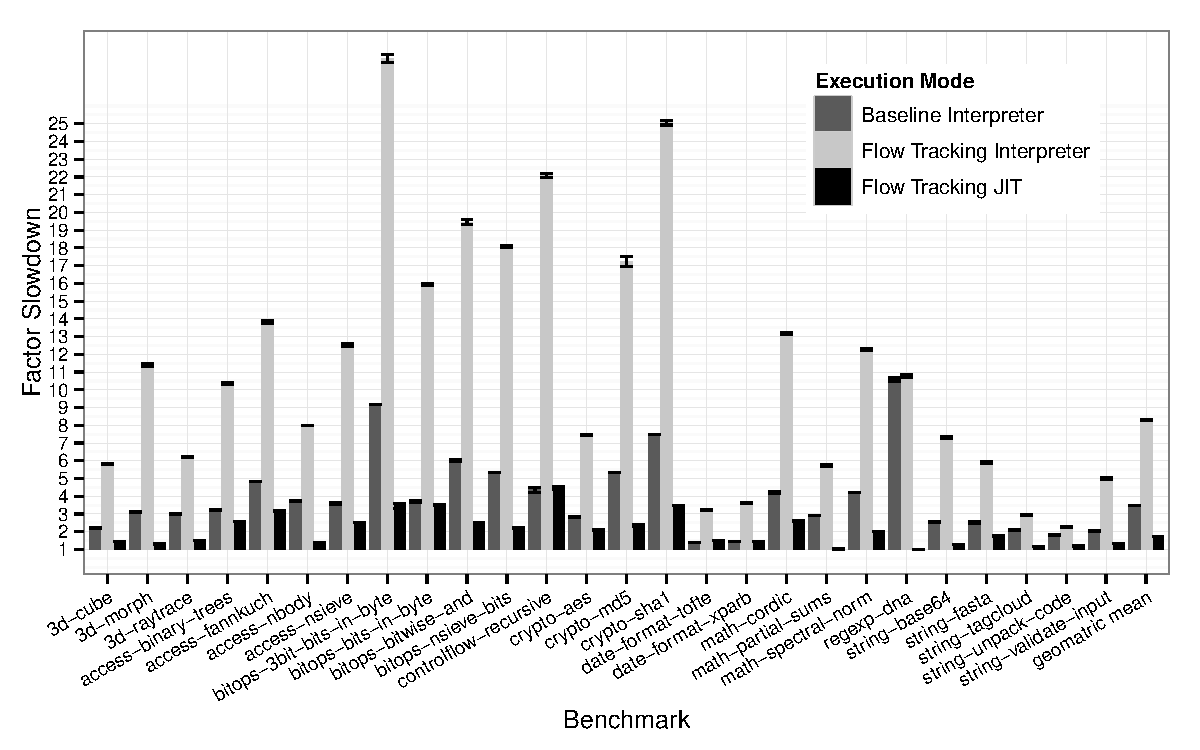
\includegraphics[width=\linewidth,keepaspectratio=true]{graphics/sunspider_plot.pdf}}
  \caption{Detailed performance for the SunSpider benchmark normalized by the \code{JavaScriptCore} JIT compiler.}
   \label{fig:sunspider-performance}
\end{figure}

\begin{figure}[ht]
  \centerline{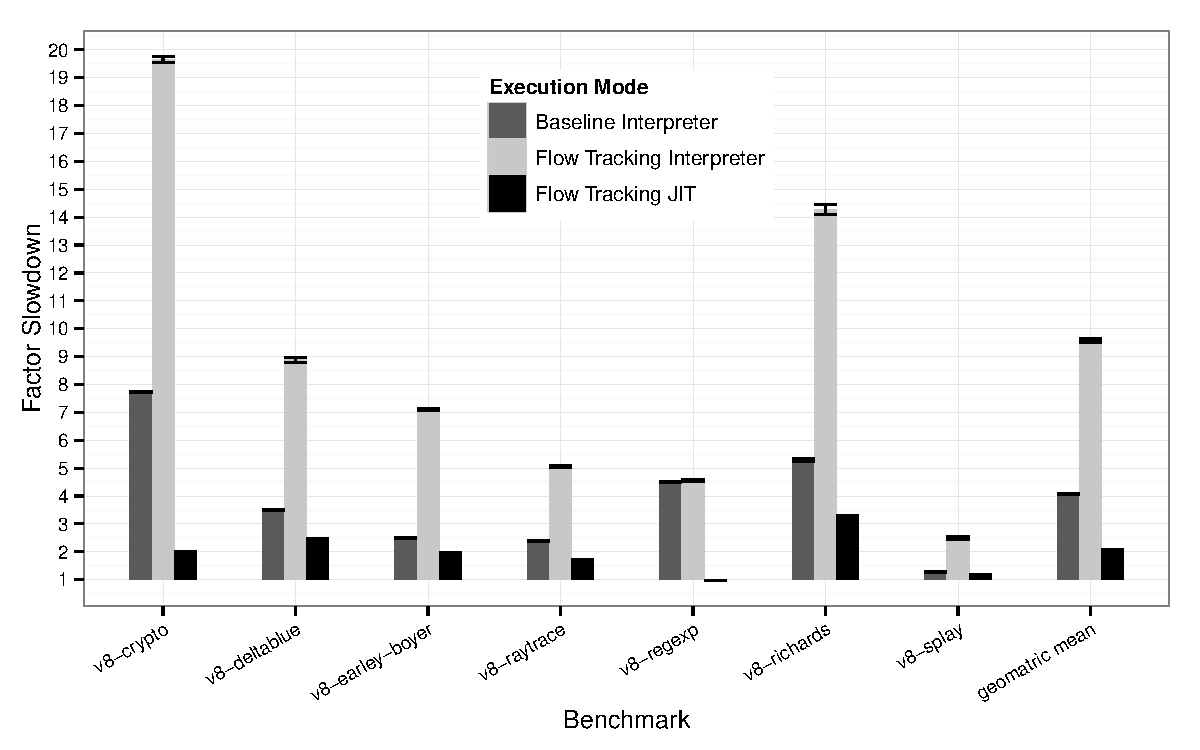
\includegraphics[width=\linewidth,keepaspectratio=true]{graphics/v8_plot.pdf}}
  \caption{Detailed performance for the V8 benchmark normalized by the \code{JavaScriptCore} JIT compiler.}
   \label{fig:v8-performance}
\end{figure}

\begin{figure}[ht]
  \centerline{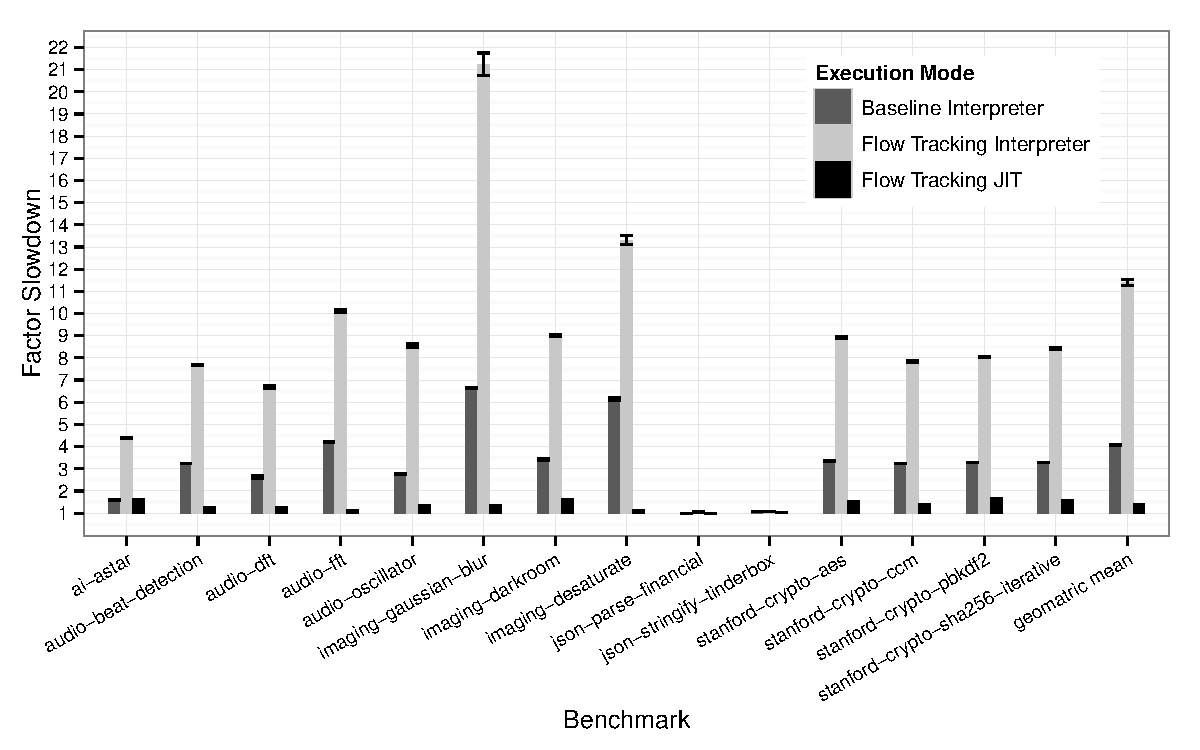
\includegraphics[width=\linewidth,keepaspectratio=true]{graphics/kraken_plot.pdf}}
  \caption{Detailed performance for the Kraken benchmark normalized by the \code{JavaScriptCore} JIT compiler.}
   \label{fig:kraken-performance}
\end{figure}

To provide a consistent basis for performance comparison, I implemented information flow tracking in WebKit's interpreter and JIT compiler using the same label encoding and supporting data structures introduced in \autoref{ch:label-propagation}.
The comparison required creating a 32-bit version of \FlowCore\ that implements inline labels, rather than the fat values discussed previously.
The benchmarks measure the performance of JIT-compiled tracking code (\JitFlow) vs. interpreter code (32-bit \FlowCore) in exclusive modes.
As illustrated in Figures~\ref{fig:sunspider-performance}, \ref{fig:v8-performance}, and \ref{fig:kraken-performance}, the average performance impact for \JitFlow\ (Sunspider~74\%, V8~108\%, and Kraken~38\%) clearly demonstrates that JIT-compiled code implementing dynamic information flow tracking outperforms the execution speed of an unmodified interpreter.
Hence, the \JitFlow\ implementation sets a new bar for dynamic information flow systems.


At the outset, I engineered and incorporated the information flow tracking logic in the JavaScriptCore interpreter, creating \FlowCore.
This effort gave me a deep understanding of WebKit's JavaScript VM and allows a comparison between the relative performance impacts of implementing dynamic information flow tracking in the interpreter vs. the JIT compiler.
Even when implementing information flow in a JIT compiler, the overhead measured as percentage relative to the baseline does not necessarily correspond to that seen when implementing the same framework within the JavaScript interpreter.
For example, the SunSpider benchmark (\autoref{fig:sunspider-performance}) shows an overhead of 137\% in the interpreter, while the JIT compiler shows only 74\%.
A full account of the performance on each individual benchmark (using the encoding and framework as described in \autoref{sec:jitflow-labelencoding}) can be found in \autoref{app:jitflow-detailedresults}.

Many of the benchmarks, such as \code{regexp} in V8 and the \code{json} family of tests in Kraken, run with essentially the same speed as the unmodified JIT compiler.
These tests perform fewer control-flow branches and make a higher percentage of native code calls compared to other tests.
Meanwhile, the \code{controlflow-recursive} test in SunSpider introduces the most overhead, at 346\%, because it has a very large number of executed branches in recursive function calls and conditional tests.
These control-flow constructs cause the dynamic information flow VM to perform additional work to maintain the control-flow stack.
Each time the VM recursively calls a function, branches on a conditional, or iterates a loop, it executes the control-flow tracking instructions (\autoref{ch:instructions}), incurring an overhead relative to an unmodified VM.

Overall, the low impact for the JIT-compiled information flow tracking logic (73\% on average, on compute intensive benchmarks) highlights the practicality of dynamic information flow as a security enhancement for the outdated JavaScript security model.

\subsubsection{Impact of Conservatively Labeling Doubles}
\label{sec:jitflow-impact-doubles}

As previously stated in \autoref{sec:jitflow-labelencoding}, the current format of doubles within WebKit does not allow directly encoding a label within the representation of a double.
All operations involving doubles implicitly carry the highest label available at the time they execute.
This conservative labeling strategy might conceal the performance drawback for benchmarks focusing on doubles.

To show that this implementation detail has little performance impact, I report the percentage of operations creating doubles vs. other \jsvalues\ for each of the three benchmark suites.
In SunSpider 4.7\% of \jsvalues\ created are doubles, while in V8 and Kraken fewer than 1\% are doubles, 0.23\% in V8 and 0.96\% in Kraken, respectively.
This ratio lets us conclude that, in those three benchmark suites, doubles account for only a small fragment of created values and therefore do not influence the overall performance impact.

\subsection{Correctness}
\label{sec:jitflow-evaluation-correctness}

To validate that the modifications \JitFlow\ makes to JavaScriptCore's JIT engine for tracking the flow of information throughout execution of a JavaScript program do not introduce any errors, we made sure that none of our modifications broke any of the Mozilla regression tests in the WebKit repository.
This suite consists of over 1,000 test cases covering core JavaScript functionality, including arrays, dates, functions, numbers, objects, regular expressions, and strings.

In addition, I wrote a suite of test cases that check the correct label propagation for the information flow tracking logic and added them to the regression suite.
These tests exercise label propagation for all of the implemented binary operations and control-flow structures: \code{if}-statements, the various loop constructs including break and continue statements, \code{eval}, and function calls.
These these tests make use of a first-class labeling framework~\cite{hennigan.etal+13} (\autoref{ch:first-class-labels}) that permits explicit application and inspection of labels within the JavaScript language itself, allowing the test cases to be incorporated into the regression suite.

\lstset{
  caption={Regression test verifying correct label propagation for additions.},
  label={list:jitflow-regressiontest},
}
\begin{jscode}
var a = (new FlowLabel("labelA"))(24);
var b = (new FlowLabel("labelB"))(12);

var res = a + b;

reportCompare(36, res, "add value incorrect.");
reportCompare(true, (labelof res).subsumes(labelof a),
              "wrong first label in add");
reportCompare(true, (labelof res).subsumes(labelof b),
              "wrong second label in add");

reportCompare((labelof res), (labelof a).join(labelof b),
              "wrong joined label in add");
\end{jscode}

\autoref{list:jitflow-regressiontest} shows one of the crafted regression tests for confirming correct label propagation.
In keeping with the other examples in this paper, this test focuses on the correct label propagation for integer addition.

The integer addition test begins by giving each of the input operands separate labels.
\Codeline{1} assigns input variable \code{a} the value \code{24} with label \code{labelA} (internally mapped to \code{0001}) and \codeline{2} assigns input variable \code{b} the value \code{12} with label \code{labelB} (internally mapped to \code{0010}).

After initialization, the test performs the addition on \codeline{4}.
To provide feedback during development, the test uses the \code{reportCompare} function, provided by the regression suite.
On \codeline{6}, it checks that the result has value \code{36} as expected.

Further sanity checking occurs on \codelines{7}{10} to ensure that the label attached to the result subsumes the label attached to each of the inputs.
Finally, on \codeline{12}, the test verifies that the label attached to the result of the addition (\code{0011}) matches the join of the labels on the operands (\code{0001|0010}).


%------------------------------------------------------------------------------------------------------
\subsection{Real World Applicability}
\label{sec:realworldapplicability}

Conforming to the capabilities of the attacker (\autoref{sec:jitflow-thirdpartycode}), this evaluation defines an information flow violation as the inequality of domains between a network data payload and the target.
When the label of the payload indicates that the data has been influenced by any origin other than the destination domain, the network request represents a communication to a foreign party, possibly an attacker-controlled server.

To verify that \JitFlow\ detects information flow violations, a web crawler automatically visits web pages and stays on each web page for 60~seconds.
The web crawler visits a randomly sampled selection 100 of the Alexa~Top~one~million~\cite{alexa} web pages.
To simulate user interaction, the web crawler fills out HTML-forms and submits the first available form on each visited page.
For all of the following results, the crawler used information flow in both the JIT compiler and the interpreter.

\begin{table*}[ht!]
\centering
\resizebox{\columnwidth}{!}{
\begin{tabular}{r|r|l|r || r|l|r}
& \multicolumn{3}{c||}{Ranked by Number of Included Domains} & \multicolumn{3}{c}{Ranked by Number of Flow violations} \\
 & \textit{Alexa Rank} & \textit{Page} & \textit{Dom.}  & \textit{Alexa Rank} & \textit{Page} & \textit{Flows}\\
\hline
1 & 556,895 & \url{prizyvnikmoy.ru} & 13 & 683,716 & \url{onefeat.com} & 295 \\
2 & 540,606 & \url{finn-dinghy.de} & 13 & 592,642 & \url{train-shop.net} & 80 \\\
3 & 438,078 & \url{mitula.ch} & 13 & 196,697 & \url{nudepornstarz.net} & 78 \\
4 & 19,658 & \url{roxio.com} & 13 & 394,557 & \url{just-eat.no} & 51 \\
5 & 999,112 & \url{printertransferroller.blogspot.com} & 12 & 889,993 & \url{sfee.gr} & 49 \\
6 & 799,519 & \url{masteringonlinemarketing.com} & 12 & 801,235 & \url{aksgonline.com} & 37 \\
7 & 683,716 & \url{onefeat.com} & 12 & 556,895 & \url{prizyvnikmoy.ru} & 35 \\
8 & 507,796 & \url{ifm-bonn.org} & 12 & 992,317 & \url{mentoring-uk.org.uk} & 30 \\
9 & 494,397 & \url{natives.co.uk} & 12 & 540,774 & \url{buildinglebow.com} & 27 \\
10 & 472,505 & \url{wcode.ru} & 12 & 834,020 & \url{tct.net.ua} & 24 \\
\hline
& & Average (of all 100 pages)& 7 & & Average (of all 100 pages)& 12 \\
\end{tabular}
}
\caption{Web pages including content from the greatest number of different domains (left) and web pages having the greatest number information flow violations (right).}
\label{tab:webstatistics}
\end{table*}

\subsubsection{Including other domains.}

Modern web applications integrate content from several different origins on the web.
Our statistics show that each of the visited web pages include an average of 7~different origins for their content.
The inline label approach lets \JitFlow\ directly encode up to 16 different domains within one label.
This technique permits an efficient encoding even for the web pages including the most content: \url{prizyvnikmoy.ru}, \url{finn-dinghy.de},  \url{mitula.ch}, and \url{roxio.com} including content from 13 domains.
These findings complement the results of Nikiforakis et al~\cite{nikiforakis.etal+12}, who visited over three million pages for their empirical study showing that more than 90\% of all pages include code from less than 15 different domains.

\subsubsection{Information flow violations}

The \JitFlow\ web crawler first visited the sample of pages using the interpreter and found 1,155 information flow violations.
The page \url{onefeat.com} had the highest observed number of violating flows, at 295.
On average, the crawler detected 12 violating flows per page in our sample (\autoref{tab:webstatistics}).

The crawler revisited the same pages the following day using the JIT compiler and found 1,173 violations.
Because the unit test cases used to develop both the interpreter and JIT compiler implementations attest to the same flow tracking and detection abilities, I attribute the 1.5\% variance between runs to dynamic page content.
For example, the page \url{newsarama.com} increased the number of content requests from 11 to 18 between the two runs, where our network monitor recorded 16 violating information flows in the interpreter and 28 information flow violations in the JIT.
Groef~et~al.~\cite{groef.etal+12} report a similar phenomenon when evaluating their system on real web pages.

The evaluation does not distinguish between malicious flows and detected flow violations due to the presence of Content Distribution Networks (CDNs), which modern web pages use for performance reasons to serve content to their users.
Before \JitFlow\ can be adopted, web site authors need a way to express allowed information flows and whitelist requests to their own CDNs.

\section{Summary}

Today, web users miss out on the increased protection afforded by information flow tracking.
All major browsers include a just-in-time compiler and vendors advertise their performance compared to competitors.
Under these circumstances, implementations of information flow tracking in the JavaScript interpreter are no longer suitable.

\JitFlow\ directly addresses the performance overhead of information flow by implementing the tracking logic in JIT-compiled code.
In spite of the prior work and analysis done to develop \FlowCore, \JitFlow\ does not ``just'' transplant interpretative tracking techniques to a JIT compiler.
Rather, it uses a different encoding that inlines the label for more efficiency with respect to space and time.
To achieve even better performance it (i) optimizes the allocation of the control flow stack to track implicit flows, (ii) it caches the top label of the control flow stack to optimize frequent accesses, and (iii) it inlines the assembly code that maintains the control flow stack to avoiding costly trampoline jumps.
Without these optimizations, a good part of the speedup from JIT compilation would have been lost.

\JitFlow\ has an average tracking overhead of 73\% relative to a baseline JIT compiler on CPU-intensive benchmarks.
On absolute terms, its performance measures more than twice as fast as the fastest known JavaScript information flow tracking interpreter.
In practice, steps such as DNS lookup, parsing and rendering, and content transmission also factor into the browser performance equation.
Consequently, using information flow tracking for realistic web browsing affects the user experience far less than CPU-intensive benchmarks may suggest.
I consider the overhead more than acceptable --- especially since users benefit from substantially increased security in return.

